\chapter{Reorganization of network architecture during reading}

\section{Motivation}

Resting-state functional connectivity is thought to provide insights into a relatively stable, ``intrinsic'' architecture. This is related to some degree to other aspects of brain structure, including structural connectivity via white matter tracts and cortical thickeness and folding \citep{Sui2014}. In Study 1, we found that global modularity is positively related to reading skill, even when controlling for verbal intelligence and motion. The inference is that global modularity is indicative of a brain organization that is more ``tuned'' to pass the information between the disparate systems needed for reading. According to one line of reasoning, modularity is indicative of a relatively stable platform for integrating multiple different areas. 

% Reorganization during tasks is important
However, it is also known that the brain can reconfigure to address new challegnes in the environment, including those of reading. It has previously been seen that, although there are many similarities within the network connectivity during rest, there also differences that arise due to task activity. One study, for example, compared a finger-tapping to working memory task. Using measures of modularity and participation coefficient, they found that within-network communication was critical for the motor task, whereas between-network communication was important for working memory \citep{Cohen2016}. This supports a hypothesis that, for a given task, there is an optimal organization, and that individuals who can better rewire their intrinsic systems to fit this organization will be more effective. 

% Effects on network organization during reading
Since reading, and especially reading comprehension, is a heavily integrative task, it must induce a much more integrated architeecture. Although global activity patterns have been described \citep{Rimrodt2009, Xu2006} global connectivity patterns, and how the measures of segregation and integration change during reading, have not. There have also been no accounts of how brain activity corresponds to measures of participation; that is, whether activation in the traditional sense corresponds to increased engagement with many areas, or if it reflects primarily local processing. This may be dependent on RSN: that is, visual areas may be more likely to perform local processing, whereas FPN areas may be more important for transferring information. 

% Reading skill
A subsequent question is whether the relationship between reading skill and network modularity \textit{while reading} should remain the same. One hypothesis is that, if cross-network communication is critical to reading, better readers should exhibit a much less modular organization while reading than poor readers. However, there is evidence from univariate analyses of brain activation that would suggest the opposite: compared to poor readers, expert readers show \textit{less} activation in many reading-related areas during reading tasks \citep{Christodoulou2014}.  In the context of interactive specialization, this is explained by the increased efficiency of information transfer within an established network. 

% This study's objectives
Investigating RSN interactions during reading is thus an excellent model system for understanding how changes to network architecture enable fluency in a specific cognitive skill. In the present study, we investigate the effects of reading comprehension on network architecture, and how it is modulated by reading skill. First, we validate our task with a traditional univariate analysis. Next, we describe the global changes to different aspects of network architecture during each condition. Then, we pinpoint which brain areas and RSNs that drive the changes to network architecture, and investgate the relationship between these changes and individual differences in reading skill. 


\section{Methods}

\subsection{Participants}

Participants were drawn from the same cohort of subjects included in Study 1, and identical inclusion criteria for both demographic and scan motion were applied. However, additional measures related to the performance of the task were levied as described below. A total of 47 unique subjects and 88 scan sessions were included in the analysis. Their demographics are described in Table \ref{table:ch3-participants}.

\begin{table}
	\renewcommand{\tabcolsep}{0.09cm}
	\centering
	\begin{tabular}{lc}
\toprule 
Measure & Subjects \\ 
\midrule 
No. Participants				& 42 \\ 
No. Scan Runs					& 164 \\ 
Gender  						& 25 F \\ 
Age at Scan 					& 10.5 (0.3)  \\ 
WASI Full-Scale IQ  			& 111.0 (16.2) \\ 
TOWRE - Total Word Efficiency 	& 104.6 (18.5) \\ 
\bottomrule 
\end{tabular}
	\caption[Participant demographics for Study 2.]{Participant demographics for Study 2. Subjects include all of those from Study 1, and three additional ones who had sufficiently high quality task-fMRI scans.}
	\label{table:ch3-participants}
\end{table}


\subsection{MRI acquisition and task design}

Participants performed up to four runs of a language comprehension task, which was crossed on two conditions: the modality of presentation (listening or reading) and the passage genre (expository or narrative). Functional MRI acquisition parameters were identical to Study 1 with the exception of scan duration, which was increased to a total of 250 dynamic volumes for each run. 

For the present analysis, only the ``reading'' scans were considered, and the effects of genre on brain activation were ignored, as they are balanced out within the majority of subjects. (6 subjects had only a single genre used for analysis.) In the following paragraphs, however, we will describe the experiment design in its entirety, as it will be relevant to subsequent analyses.

Each fMRI run had two baseline conditions: a modality-specific baseline task and a resting-state block with a fixation cross. At the conclusion of the comprehension portion of each experiment, two images were presented, and subjects were asked to decide if the image was related to the passage. (e.g., Is a picture of a cake with candles related to a story about a birthday party?) The order and duration for each block varied slightly across runs but was approximately: paragraph 1 (60 s), baseline 1 (60 s), paragraph 2 (60 s), baseline 2 (60 s), and resting-state (270 s). Total scan time was 550 s for each run. See Fig. \ref{fig:ch3-task-design} for a schematic describing the visual task.

\begin{figure}[t]
	\centering
	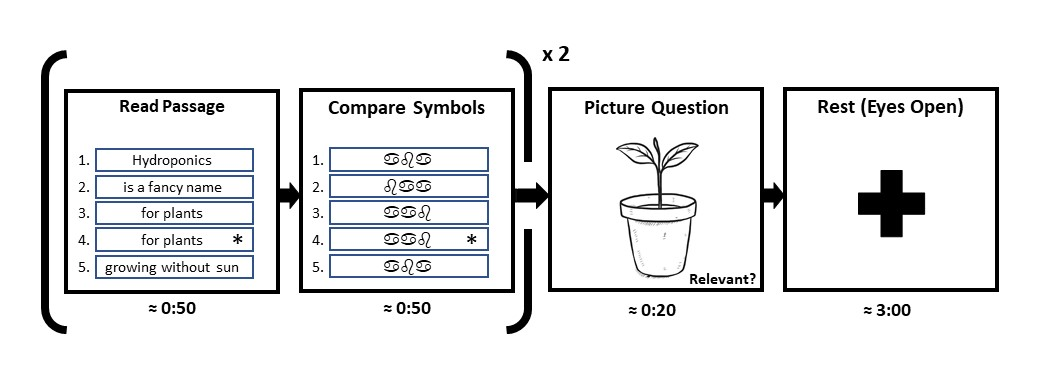
\includegraphics[width=6in]{ch3-task-design}
	\caption[Schematic of the reading comprehension task.]{Schematic of the reading comprehension task. Subjects were presented two blocks of passage reading and a symbol comparison tasks, which were followed by a brief comprehension question and a resting block.}
	\label{fig:ch3-task-design}
\end{figure}

To create a more naturalistic reading experience than single word presentation \citep{Rayner1998}, passages were presented in syntactic phrases ranging from 1-7 words in length. The interval between each stimulus was jittered to allow for event-related analyses (range: 275 – 4000 ms), although these effects were not examined here.

The sensory baseline condition was altered according to modality. For the reading runs, three non-alphanumeric symbols were displayed horizontally (two types), and their presentation time was matched to the passage phrases. Spacing between symbols was randomly alternated to replicate the variable phrase lengths in the passage condition. For the listening runs, three tones (two frequencies) were played in sequence, with a new set of tones beginning at the same intervals as the corresponding passage presentation. 

To monitor attention, 4 to 8 percent of the stimuli within each passage or attention block were randomly repeated on two consecutive screens.  Participants pressed a button with their right thumb when they detected a repeated phrase, symbol or tone configuration. Additionally, at the conclusion of each passage, a picture was presented on the screen, and subjects were asked to identify whether the picture had any relationship to the passage (e.g., a picture of a mushroom for a passage about fungi). 

To assess performance, we analyzed three measures: in-scanner attention, in-scanner comprehension, and post-scan recall. To assess attention for the ``repeated stimulus'' task, we used the $D`$ summary measure. It is calculated as:

$$
D^\prime = Z_{true\ positive} - Z_{false\ positive}
$$

The in-scanner comprehension measure was the number (0,1,2) of questions correclty answered. To assess recall, each child was asked to recite as much of the passage as they could remember, and their answers were mapped to actual phrases present in the chapter. Individual scan runs with a $D`$ value less than 2 were excluded from analysis.

In total, there were 4 passages (2 listening and 2 reading), each leveled to a third grade difficulty level and balanced on word measures such as concreteness and cohesiveness.  All subjects were trained on the task in a mock scanner prior to the actual scan. 


\subsection{Activation analyses}

Whole-brain fMRI analyses were performed using tools from the FMRIB Software Library (version 5.0.9). For each session, the following pre-processing steps were performed:  slice-time correction, motion correction to the initial fMRI volume, high-pass filtering at 0.08 Hz, boundary-based registration to the subject's structural image, and normalization to 2 mm MNI 152 standard space. To mitigate the effects of motion on our analyses, we regressed out 6 continuous motion parameters and scrubbed out outlier volumes. We defined an outlier volume as any in which the root-mean-square framewise displacement exceeded 0.7 mm. We removed scan runs where more than 20 percent of the fMRI volumes were considered outliers.

All task conditions were convolved with the double-gamma hemodynamic response function to generate design matrices for each fMRI run. Two first-level contrasts were of interest: the main effect of passage comprehension (``Reading vs. Rest''), and the contrast of passage comprehension vs. the sensory baseline (``Reading vs. Attention''). Repeated stimuli and the picture comprehension task were modelled out.

Reading effects were estimated at the subject-level using fixed effects analysis. These were carried over into group-level analyses using non-parametric methods implemented in FSL’s \textit{randomise} tool with threshold-free cluster enhancement. For each group-level analysis, we performed 5000 permutations and report results with \textit{p} \textless 0.05. 

To understand our univariate results as a function of system-level activation, we also extracted activation values from each of the 264 connectome nodes, and summarized the activity of each ``intrinsic'' RSN.

\subsection{Network analyses}

For graph theory analyses, network estimation was performed in the \textit{Conn: Functional Connectivity Toolbox} (version 17f) \citep{WhitfieldGabrieli2012}. As before, for each scan run, the BOLD activity at each node was denoised using the anatomical CompCorr method, which regresses out background noise from white matter and cerebrospinal fluid tissue. We also regressed out 12 continuous measures of motion were also included, all outlier timepoints, and the effect of all task conditions (``Reading'', ``Attention'', ``Rest''). The timeseries was then high-pass filtered at 0.01 Hz.

Whole-brain connectomes for each condition were created by estimating the functional connectivity between each node using a weighted general linear model. For connection-level analyses, these values were compared directly across subjects and conditions. For graph theory analyses, the array of all node connections was thresholded to keep the top 5 percent of connections, resulting in a much sparser representation. This threshold was also tested at ranges from 2 percent to 10 percent. These arrays were then characterized using the previously described graph theory measures: modularity, participation coefficient, and path length.


\section{Results}

47 subjects (88 scan runs) met the attention and motion criteria for inclusion in the analysis. (5 subjects and 15 scan runs were excluded.) The distribution of performance and motion criteria are illustrated in Figure \ref{fig:ch3-task-performance}. 

\begin{figure}[t]
	\centering
	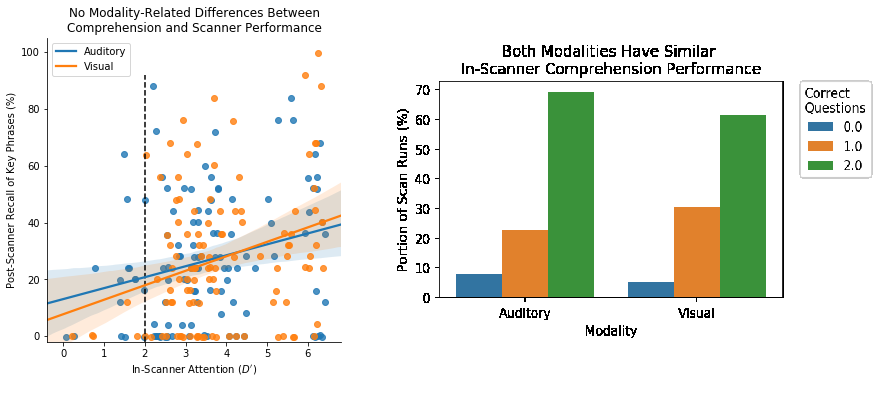
\includegraphics[height=3in]{ch3-task-performance}
    \caption[Description of scan motion quality and task performance.]{Scatterplot summarizing the relationship between scan motion quality and task performance. The $D^\prime$ score measures performance based on both active (correctly identifies repeats) and passive (few false alarm clicks) metrics. The frame-wise displacement measure also accoutns for outlier volumes, which are regressed out during analysis.}
	\label{fig:ch3-task-performance}
\end{figure}

\subsection{Activation results}

A range of language-related areas were activated during reading comprehension (Fig. \ref{fig:ch3-reading-brain-activation}). Compared to the attention baseline, reading-related activation spanned the inferior frontal gyrus, angular gyrus, premotor cortex, middle temporal gyrus and the superior frontal gyrus. Activation patterns were robustly present on both hemispheres but extended further and with greater intensity on the left hemisphere. There were also a number of areas that were more active in the sensory and resting state, especially in the dorsal attention network and anterior dorsolateral prefrontal cortex.

\begin{figure}[t]
	\centering
	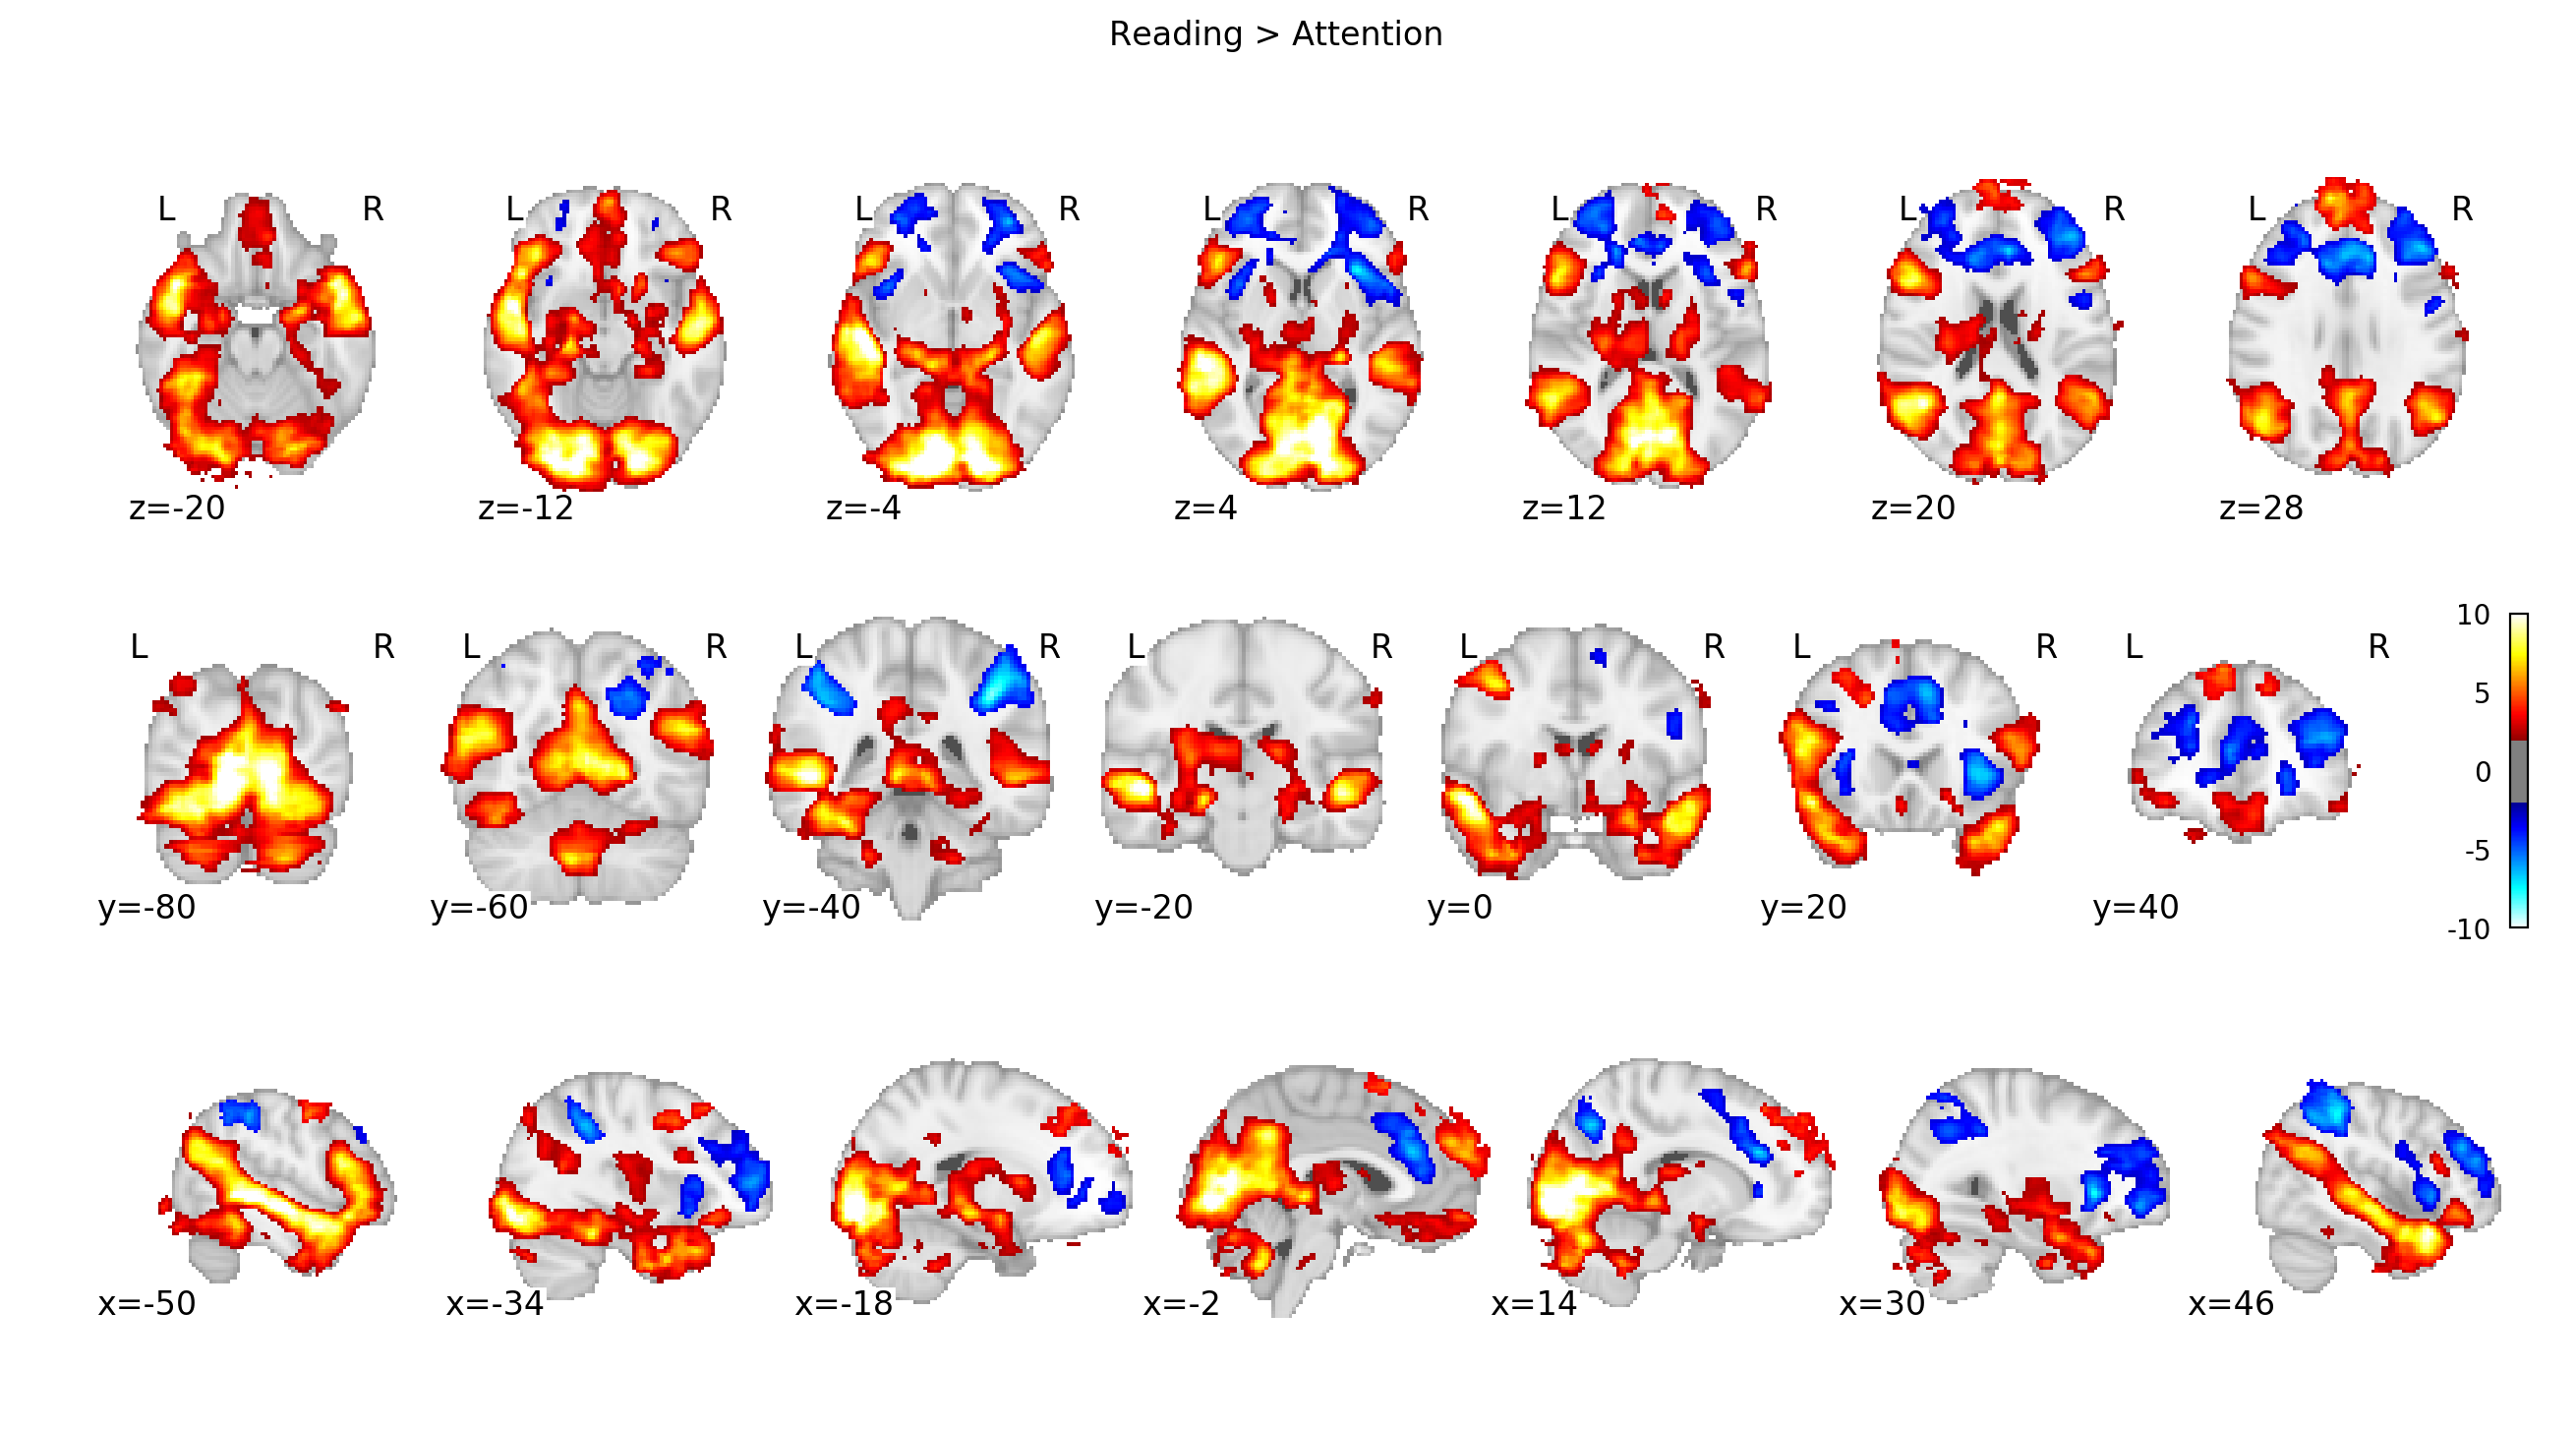
\includegraphics[width=6in]{ch3-reading-brain-activations}
    \caption[A range of language-related areas were activated during reading comprehension.]{A range of language-related areas were activated during reading comprehension. The above figures show axial, coronal and sagittal views of the ``reading vs. attention'' activation contrast. Reading-related activations span expected areas, including left fusiform, middle temporal and inferior frontal gyri, but also extend into right hemisphere homologues and the cerebellum. Results are thresholded at $p < 0.05$ using threshold-free cluster enhancement (5000 permutations).}
	\label{fig:ch3-reading-brain-activations}
\end{figure}

To understand RSN-level trends in activation, We also examined the results when projected onto the 264 nodes in the connectome parcellation. Compared to the resting baseline, the ventral attention, visual and default mode networks had the greatest number of ``activated'' nodes. It is also notable that the ``uncertain'' nodes were highly engaged, possibly reflecting the important role of functionally diverse regions in the execution of reading comprehension. On the other end, the memory retrieval, salience and cingulo-opercular networks exhibited decreased activity compared to rest. See Fig. \ref{ch3-reading-connectome-activations} for a diagram of these activations by RSN. 

\begin{figure}[t]
	\centering
	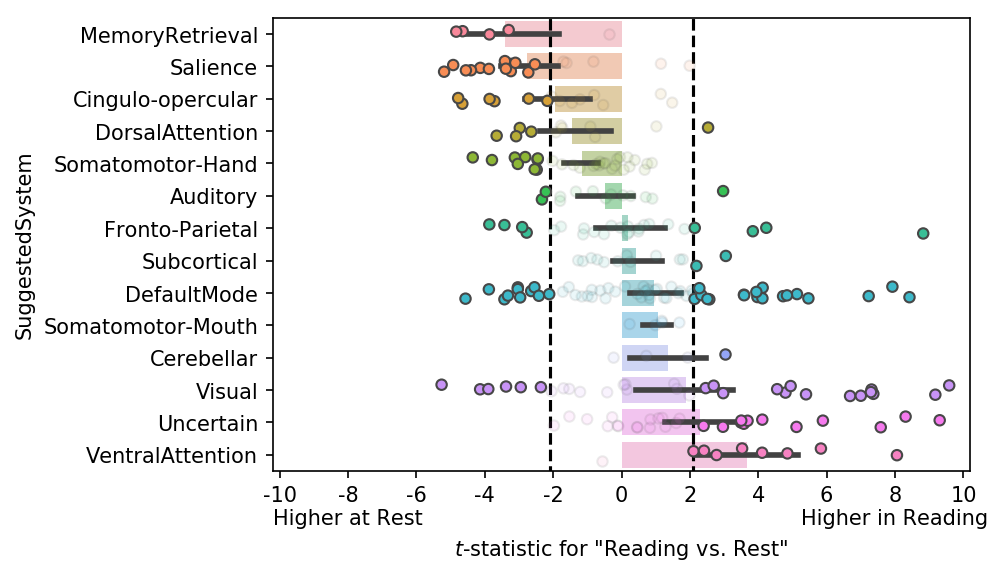
\includegraphics[height=3in]{ch3-reading-connectome-activations}
    \caption[Distribution of reading-related activity among RSN nodes.]{Distribution of reading-related activity among connectome nodes, grouped by RSN. Each point represents a single node, while bars represent the aggregate mean for each RSN. Visual and ventral attention networks showed the most network-level activity in reading, although large portions of the default mode and fronto-parietal network were also robustly related. Cingulo-opercular, memory retrieval and salience networks showed decreases. Dashed lines represent $p < 0.05$, uncorrected.}
	\label{fig:ch3-reading-connectome-activations}
\end{figure}


\subsection{Network results}

Next, we examined changes to global network architecture. Figure \ref{fig:ch3-comprehension-graph-theory-all} summarizes the subject-level changes in modularity, participation coefficient, and path length. Overall, the effect was one of increased integration across RSNs during reading comprehension. Relative to rest, both reading comprehension and the sensory baseline reduced the global modularity and increased the participation coefficient. The magnitude of the effect in reading comprehension was also greater than that of the sensory condition. The path length within each RSN did not significantly change across condition, suggesting that the modular organization of the brain was not disrupted; the RSN parcellation used was still a good fit. However, there were significant increases in the between-RSN path length corresponding to greater efficiency of transferring information between these disparate systems.

\begin{figure}[t]
	\centering
	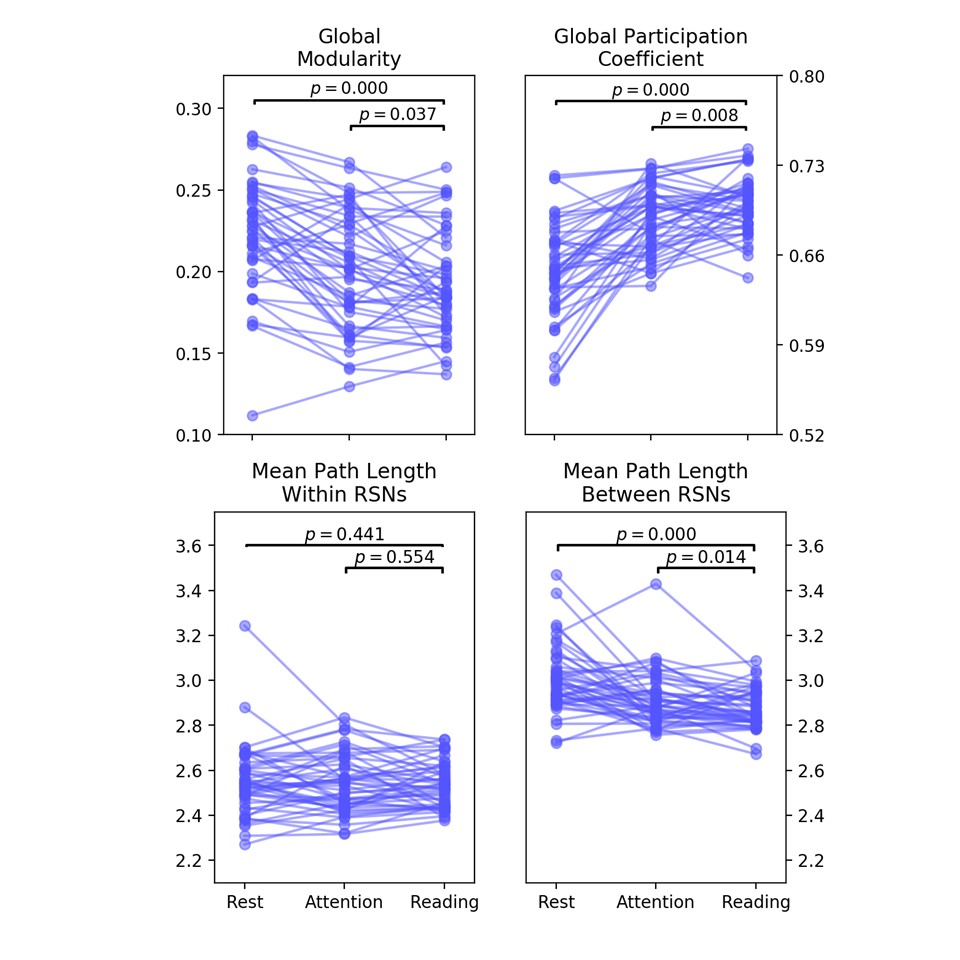
\includegraphics[width=5.3in]{ch3-comprehension-graph-theory-all}
    \caption[Reading induces more integrated global network architecture.]{Reading induces more integrated global network architecture. Compared to rest and the baseline attention task, reading comprehension increased global measures related to RSN integration. Notably, the only measure not significantly changed during task was the within-RSN path length.}
	\label{fig:ch3-comprehension-graph-theory-all}
\end{figure}

Network-level trends in task-evoked differences to graph theory measures were largely related to global trends, and they are presented in Figure   \ref{fig:ch3-rsn-condition-effects}. However, a few findings are worth noting: compared to rest, reading was marked by large decreases in modularity of the visual, dorsal attention and default mode netowrks; however, the increases to participation coefficient were global. Compared to the attention task, network-level changes were more modest, and the global differences were driven by reduced modularity in the default mode and fronto-parietal networks, an increased participation of memory retrieval and default mode networks.

% Need to add significance asterisks, thresholds, fix legend (attention, reading) and reduce white sapce
\begin{figure}[t]
	\centering
	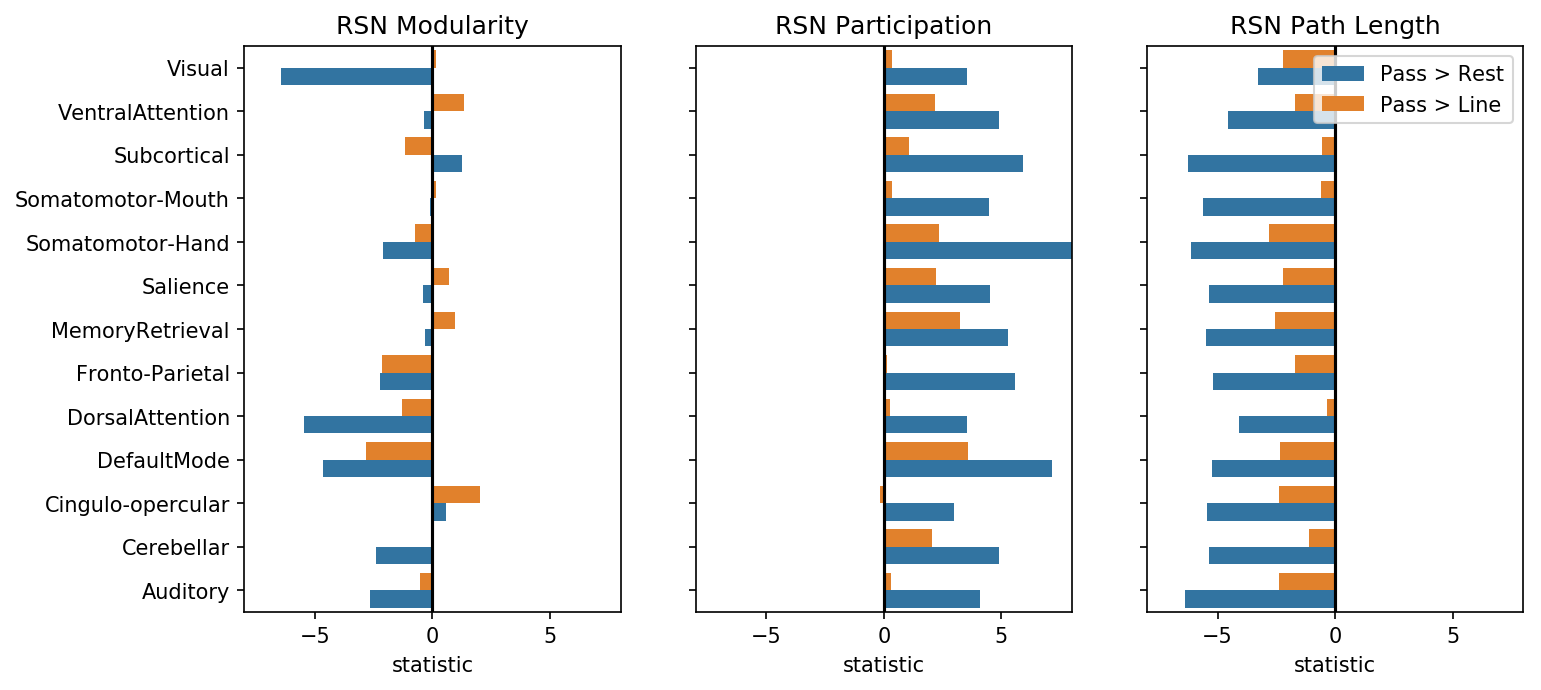
\includegraphics[width=6in]{ch3-rsn-condition-effects}
    \caption[RSN-level trends in task-evoked networks.]{RSN-level trends in task-evoked networks. Network-level trends in task-evoked differences to graph theory measures were largely related to global trends.}
	\label{fig:ch3-rsn-condition-effects}
\end{figure}

We also compared the two approaches to assess whether greater activity was connected to greater participation across the network. We found that nodes that were more activated in reading relative to rest tended to be those which were not hub-like ($r = -0.434$, $p < 0.001$). In fact, those areas that were most hub-like tended to show the least ``activity'' from a univariate standpoint (see Fig. \ref{fig:ch3-node-participation-to-activation}). 

\begin{figure}[t]
	\centering
	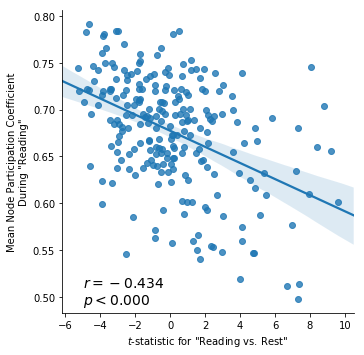
\includegraphics[width=4in]{ch3-node-participation-to-activation}
    \caption[Activity is anti-correlated with participation coefficients.]{Compared to rest and baseline attention tasks, reading comprehension increased measures related to RSN integration.}
	\label{fig:ch3-node-participation-to-activation}
\end{figure}

% To investigate interactions between networks, rather than simply general behavior of the networks, we summarized the average shortest path length between each network. This provides a gross measure of how close any two networks are. A node-level diagram of these changes between rest and comprehension is presented in Figure \ref{ch3-modality-node-distance}. 

% \begin{figure}[t]
% 	\centering
% 	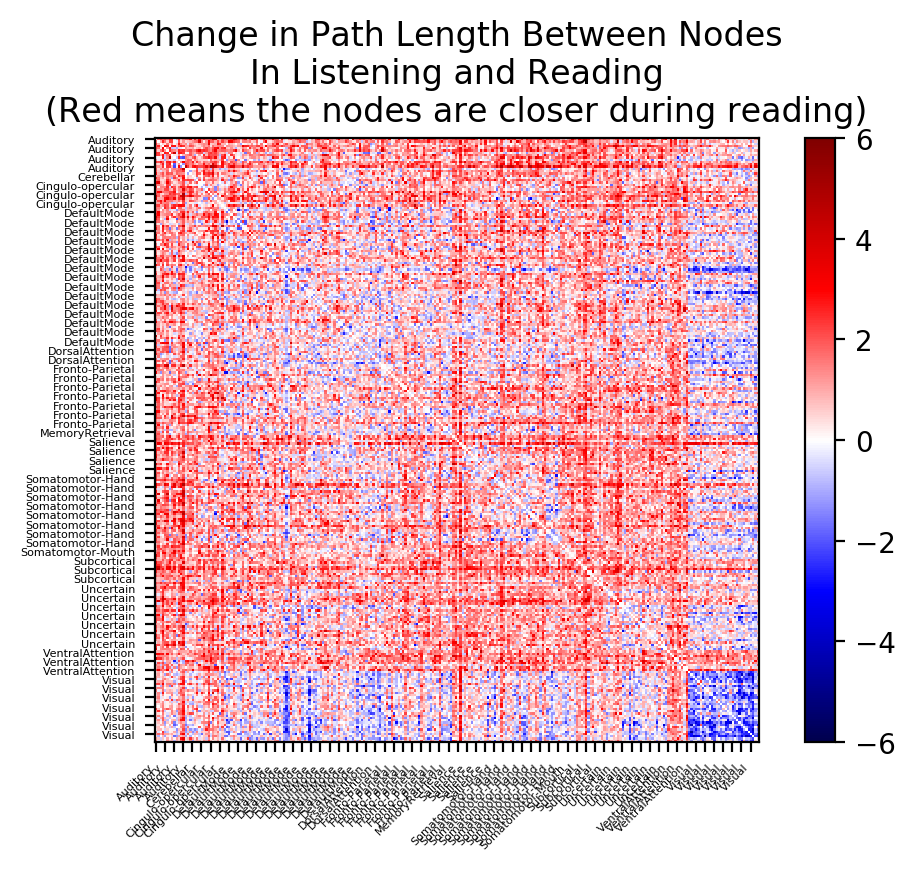
\includegraphics[height=3in]{ch3-modality-node-distance}
%     \caption[Language induces more integrated global network architecture.]{Compared to rest and baseline attention tasks, reading and listening increase measures related to global RSN integration.}
% 	\label{fig:ch3-modality-node-distance}
% \end{figure}

Investigating these graph theory measures at the level of RSN provides insight as to which networks are driving the changes in integration. When comparing comprehension differences to rest, for example, we can see that globally connectivity increases (Fig. \ref{fig:ch3-comprehension-reorganization}. During rest, however, there is increased connectivity within default mode network and visual networks. As would be expected, the visual network undergoes large changes in reading: specifically, there is a large decrease in visual-visual connectivity. 

\begin{figure}[t]
	\centering
	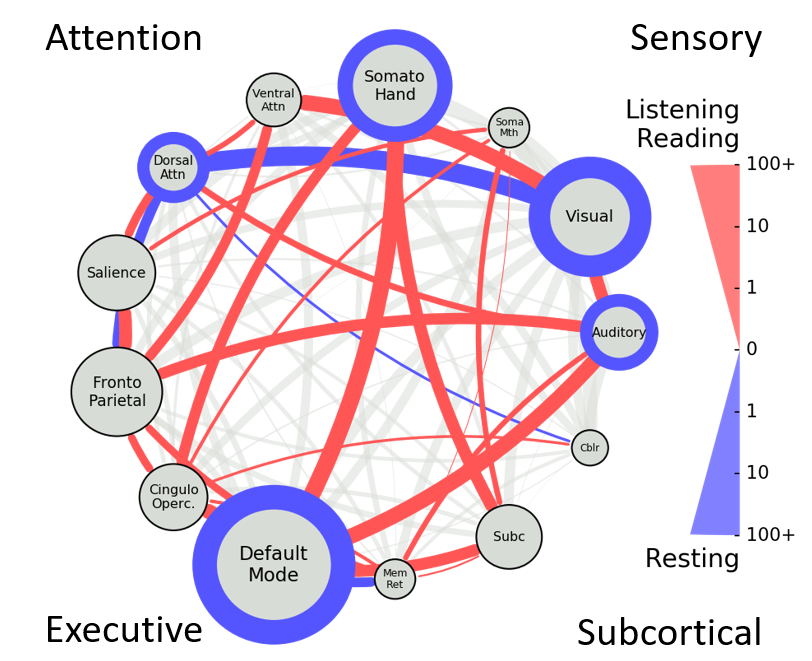
\includegraphics[height=4.5in]{ch3-comprehension-reorganization}
    \caption[Changes in number of connections within and between networks.]{Changes in number of connections within and between networks.}
	\label{fig:ch3-comprehension-reorganization}
\end{figure}

Finally, we sought to address the question of whether better readers more likely to have decreased modularity during reading. As before 

\begin{figure}[t]
	\centering
	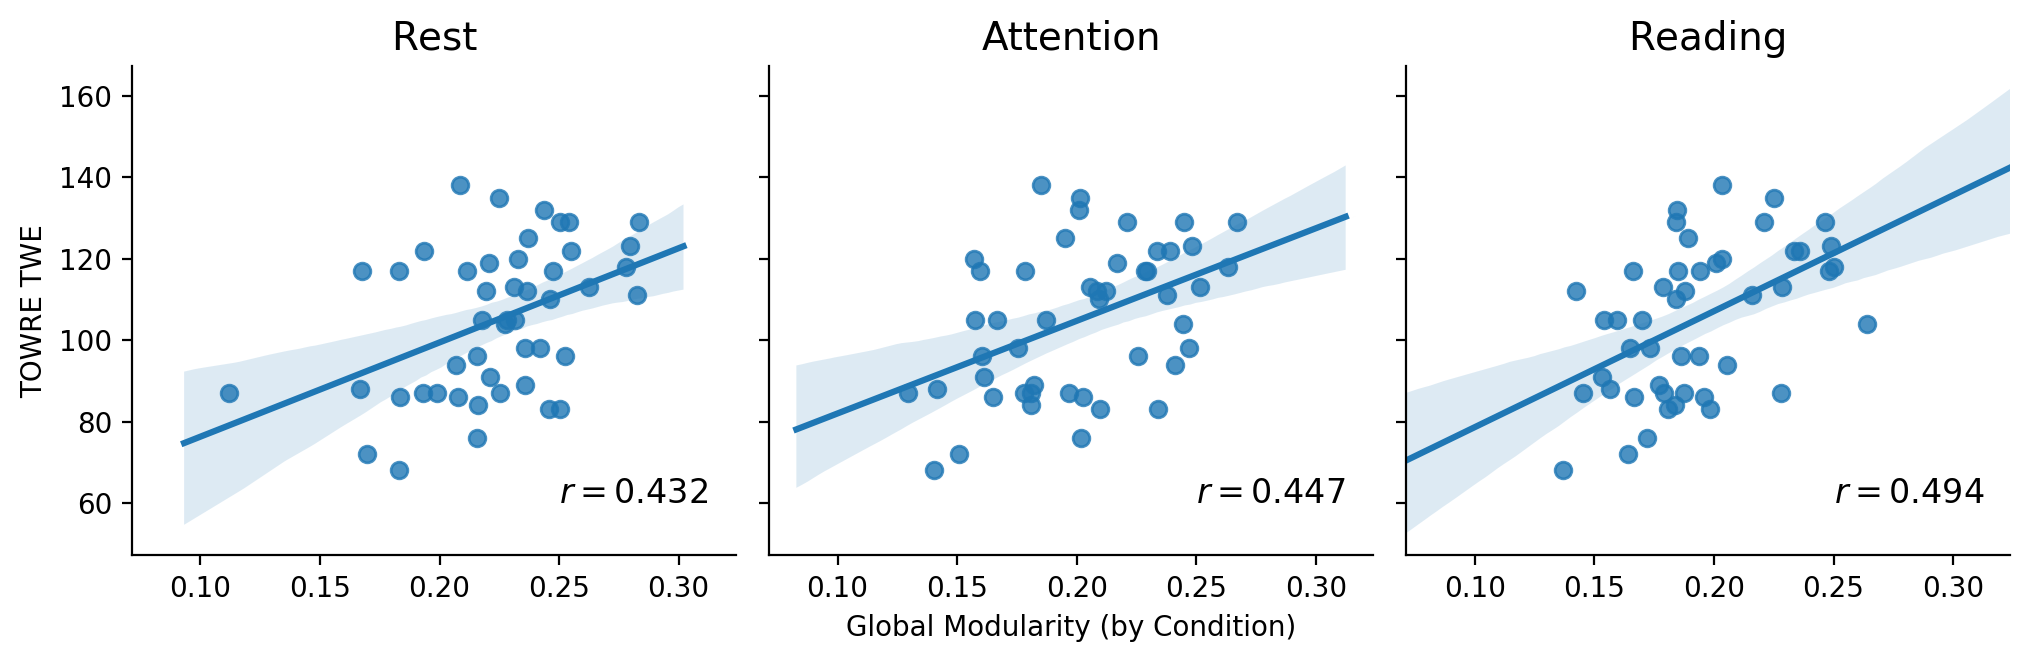
\includegraphics[width=6in]{ch3-modularity-reading-by-condition}
    \caption[Higher modularity in any condition is related to reading skill.]{Higher modularity in any condition is related to reading skill. Greater integration between}
	\label{fig:ch3-modularity-reading-by-condition}
\end{figure}


\section{Discussion}

The current study sought to determine to what extent important aspects of the brain's network architecture change during reading. The results suggest that the maintenance of an efficient network organization, i.e. one in which brain areas form clusters connected by hub regions, is important for skilled reading, even as between-network connectivity increases. To our knowledge, this is the first time the relationship between modularity and hubness to reading skill has been described, adding to a foundation of work built on other connectivity methods.

% Distribution of activity among different RSNs
One insight gained in this study is that much of the ``reading network'' falls in domain-general RSNs such as the attention and executive networks. While these areas perform a specific function in reading, they are also often involved in other processes. For example, the dorsal attention network encompasses the visual word form area, an area that has been the subject of much interest and debate in reading and dyslexia research \citep{McCandliss2003}. It is probable that this area is so important in reading not only because it is connected to language areas \citep{Bouhali2014}, but also because it is tightly tied to other areas that control goal-directed attention \citep{Vogel2014}. Koyama and colleagues found that children with a historical diagnosis of dyslexia had persistent de-coupling of the DAN compared to typical readers regardless of remediation status \citep{Koyama2013}. Vogel et al. found that reading ability in typical children and adults (including decoding and passage comprehension ability) predicted increased correlations between the visual word form area and the DAN \citep{Vogel2012a}. The nesting of this orthographic-processing area within the DAN is thus important to its role in reading.

% Changes to global modularity, but no changes  to reading correlation
In terms of global network effects, we found that tasks reduced global measures of modularity and increasd measures of between-RSN communication, including participation coefficient and path length. This was most apparent in the visual RSN, which was characterized by a major decrease in modularity compared to rest. Our findings support a model in which the brain adopts a modular architecture at rest then changes during tasks to better accommodate the structure. An efficient small-world organization in the resting brain requires a modular network architecture, which was tied here to better performance in reading. This relationship was particularly high in the visual, default mode, cingulo-opercular networks. 

% Network level effects + correlation with reading
It is not yet possible to say whether modularity within these specific RSNs correlates most highly with reading because of their functional roles in reading processes or whether they simply capture global trends better than other networks. There is some reason to suspect specificity, however. In studies of remediation-induced changes to connectivity, increased connectivity within the visual network \citep{Koyama2013} and cingulo-opercular network \citep{HorowitzKraus2015} have predicted reading improvement in dyslexic children. The default mode network, on the other hand, supports a wide range of cognitive processes important for comprehension, including theory of mind, narrative processing, and autobiographical recall \citep{Buckner2008, AbdulSabur2014}, and its cohesiveness during resting-state has been used to investigate other disorders \citep{Uddin2008}. Future work will need to examine not just the internal connectivity, but the relationships between these networks during reading and at rest. The default mode network, for example, is typically anti-correlated with "task-positive" networks such as the fronto-parietal network. A high degree of anti-correlation has been reported to be important for performance on a variety of cognitive processes \citep{Fox2005, Keller2015}, but recent work suggests that high modularity and connectivity of the default mode during higher-level cognition is fundamental to processes relying on self-referential and memory retrieval processes, such as those found in language \citep{Vatansever2015}. The dynamics behind these interactions will be important for further establishing a framwork for investigating the roles of specific networks during reading. 

% Participation coefficient
It is perhaps surprising to see primarily global effects of condition on the participation coefficient. Other work has found that certain networks, such as the fronto-parietal network are responsible for task-switching \citep{Cole2013}. Previous research have also noted that brain regions that have been found to be abnormal in dyslexia localize on high-hub regions \citep{Bailey2018}. However, the literature on dyslexia may be insightful here: several of these regions, including the inferior frontal gyrus and inferior parietal lobule have been found to be both active in some studies and inactive in others. It is perhaps, then, an abnormality in the system rather than underactivation. The anti-correlation between task activity and participation coefficient highlights the complementary nature of network analysis with activation analyses. What it suggests is that ``hub'' regions have a primary role as connectors, whereas only in some cases are regions active and highly participatory. 
% Show picture of PC on x-axis and activity on y-axis


% The additional findings that hubs areas are key in dyslexia are not surprising: dyslexia has often been thought to be a disorder of combining information across different functional systems, and in the context of connectomics, hub areas play a privileged role in mediating information flow between RSN’s. For example, the posterior temporal sulcus connects visual and auditory networks by binding letters to sounds \citep{Blau2010, VanAtteveldt2009} and the inferior frontal gyrus has many different subdivisions supporting language parsing and manipulation \citep{Hagoort2005}. However, casting dyslexia dysfunction into a connectomics perspective opens up new hypotheses and research avenues. For example, the brain areas of interest and neuroimaging metrics can be unified across other developmental disorders, including ADHD, specific language impairment and autism \citep{Stam2014}. Another benefit is that it opens up many more avenues for investigating dyslexia using functional and diffusion MRI, which can be performed in younger children and without administering a cognitive task. 

Taken together, these results suggest that the network architecture of the brain is quite stable across task-evoked and resting states, lending further credence to assertions that it measures someting intrinsic and stable. However, between-netowkr connectivity does increase the connectivity between different RSNs, and the role of the network region (participation coefficient0 is importamy be related to its  role in the system. That is, task-negative areas, including those in the default mod network, were more likely to habe higher participation coefficients. )